\documentclass{scrartcl}
 
\usepackage[utf8]{inputenc}
\usepackage[T1]{fontenc}
\usepackage{lmodern}
\usepackage[ngerman]{babel}
\usepackage{amsmath}
%\usepackage{enumitem}
\usepackage{pgfplots}
\usepackage{enumerate}
\usepackage{caption}
\usepackage{amssymb}

\title{Übungen - Signale und Systeme 2}
\author{Markus Kessler | Mathias Lechner | Martin Wührer}
\date{SS14}

%Speziell der Befehl \leftn wird oft benötigt, da ansonsten x [ entsteht.
\newcommand*\leftn{\negthinspace\left}
\newcommand*\rightn{\right\negthinspace}

\begin{document}
\maketitle
\section*{Aufgabe 1.1}

\subsection*{Angabe}
 
Für das zeitbegrenzte Signal
	\begin{equation*}
		x\leftn[n\right] = \left\{\begin{array}{cl} 0, & n<0\\n, & 0\le n\le 10\\0, & n>10 \end{array} \right.
	\end{equation*}
zeichnen Sie folgende Signale:
	\begin{enumerate}[a)] 
		\item $y\leftn[n\right] = x\leftn[n+5\right]$
		\item $y\leftn[n\right] = x\leftn[-n+5\right]$
		\item $y\leftn[n\right] = x\leftn[2n\right]$
		\item gerades und ungerades Teilsignal von $x\leftn[n\right]$
		\item $y\leftn[n\right] = x\leftn[n+10\right]+x\leftn[-n+10\right]-10\delta\leftn[n\right]$
	\end{enumerate}

\subsection*{Lösung}
Die gegebene Funktion $x\leftn[n\right]$:\\
\begin{center}
\resizebox{200pt}{150pt}{%
	\begin{tikzpicture}
		\begin{axis}[
			domain=-10:20,
			axis x line=bottom,
			axis y line=middle,
			ylabel = {$x\leftn[n\right]$},
			xlabel = $n$,
       		xtick={-10,-5,...,20},
			]
			\addplot+[ycomb,blue,thick,domain=-10:-1,samples=10,mark=o] {0};
			\addplot+[ycomb,blue,thick,domain=0:10,samples=11,mark=o] {x};
			\addplot+[ycomb,blue,thick,domain=11:20,samples=10,mark=o] {0};
			
			\draw[blue,thick] ({axis cs:10,10}) -- ({axis cs:10,0});
		\end{axis}
	\end{tikzpicture}
}\end{center}\clearpage
\textbf{a)} $\mathbf{y\leftn[n\right] = x\leftn[n+5\right]}$\\
\begin{center}
\resizebox{200pt}{150pt}{%
	\begin{tikzpicture}
		\begin{axis}[
			domain=-10:20,
			axis x line=bottom,
			axis y line=middle,
			ylabel = {$y\leftn[n\right]=x\leftn[n+5\right]$},
			y label style={at={(-0.1,0.95)}},
			xlabel = $n$,
       		xtick={-10,-5,...,20},
			]
			\addplot+[ycomb,blue,thick,domain=-10:-6,samples=5,mark=o] {0};
			\addplot+[ycomb,blue,thick,domain=-5:5,samples=11,mark=o] {x+5};
			\addplot+[ycomb,blue,thick,domain=6:20,samples=15,mark=o] {0};
			
			\draw[blue,thick] ({axis cs:5,10}) -- ({axis cs:5,0});
		\end{axis}
	\end{tikzpicture}
}\end{center}
\textbf{b)} $\mathbf{y\leftn[n\right] = x\leftn[-n+5\right]}$\\
\begin{center}
\resizebox{200pt}{150pt}{%
	\begin{tikzpicture}
		\begin{axis}[
			domain=-10:20,
			axis x line=bottom,
			axis y line=middle,
			ylabel = {$y\leftn[n\right]=x\leftn[-n+5\right]$},
			xlabel = $n$,
       		xtick={-10,-5,...,20},
			]
			\addplot+[ycomb,blue,thick,domain=-10:-6,samples=5,mark=o] {0};
			\addplot+[ycomb,blue,thick,domain=-5:5,samples=11,mark=o] {-x+5};
			\addplot+[ycomb,blue,thick,domain=6:20,samples=15,mark=o] {0};
			
			\draw[blue,thick] ({axis cs:-5,10}) -- ({axis cs:-5,0});
		\end{axis}
	\end{tikzpicture}
}\end{center}
\textbf{c)} $\mathbf{y\leftn[n\right] = x\leftn[2n\right]}$\\
\begin{center}
\resizebox{200pt}{150pt}{%
	\begin{tikzpicture}
		\begin{axis}[
			domain=-10:20,
			axis x line=bottom,
			axis y line=middle,
			ylabel = {$y\leftn[n\right]=x\leftn[2n\right]$},
			y label style={at={(-0.1,1)}},
			xlabel = $n$,
       		xtick={-10,-5,...,20},
			]
			\addplot+[ycomb,blue,thick,domain=-10:-1,samples=10,mark=o] {0};
			\addplot+[ycomb,blue,thick,domain=0:5,samples=6,mark=o] {2*x};
			\addplot+[ycomb,blue,thick,domain=6:20,samples=15,mark=o] {0};
			
			\draw[blue,thick] ({axis cs:5,10}) -- ({axis cs:5,0});
		\end{axis}
	\end{tikzpicture}
}
\end{center}
\pagebreak

\textbf{d) gerades und ungerades Teilsignal von} $\mathbf{x\leftn[n\right]}$\\
Für die geraden und ungeraden Teile definieren wir zuerst allgemein:
\[
	x\leftn[n\right]=x_g\leftn[n\right]+x_{ug}\leftn[n\right]
\]
Nun erhalten wir durch umformen:
\begin{align*}
\text{Gerades Signal: } x_g\leftn[n\right]&=\frac{1}{2}\left(x\leftn[n\right]+x\leftn[-n\right]\right), \forall n\\
\text{Ungerades Signal: } x_u\leftn[n\right]&=\frac{1}{2}\left(x\leftn[n\right]-x\leftn[-n\right]\right), \forall n
\end{align*}
Daraus lassen sich nun die geraden und ungeraden Teilsignale berechnen (einfaches Einsetzen):\
\begin{figure}[!h]	%1.2) d - Gerades Teilsignal
\centering
	\begin{tikzpicture}[scale=0.8]
		\begin{axis}[
			domain=-10:20,
			axis x line=bottom,
			axis y line=middle,
			ylabel = {$x_g\leftn[n\right]=\frac{1}{2}\left(x\leftn[n\right]+x\leftn[-n\right]\right)$},
			y label style={at={(0.2,1.2)}},
			xlabel = $n$,
       		xtick={-10,-5,...,20},
			]
			\addplot+[ycomb,blue,thick,domain=-10:0,samples=11,mark=o] {-x/2};
			\addplot+[ycomb,blue,thick,domain=1:10,samples=10,mark=o] {x/2};
		\end{axis}
	\end{tikzpicture} \caption*{Gerades Teilsignal}
\end{figure}
\begin{figure}[!h]	%1.2) d - Ungerades Teilsignal
\centering
	\begin{tikzpicture}[scale=0.8]
		\begin{axis}[
			domain=-10:20,
			axis x line=middle,
			axis y line=middle,
			ylabel = {$x_u\leftn[n\right]=\frac{1}{2}\left(x\leftn[n\right]-x\leftn[-n\right]\right)$},
			y label style={at={(0.2,1.2)}},
			xlabel = $n$,
       		xtick={-10,-5,...,20},
			]
			\addplot+[ycomb,blue,thick,domain=-10:10,samples=21,mark=o] {x/2};
		\end{axis}
	\end{tikzpicture} \caption*{Ungerades Teilsignal}
\end{figure}\clearpage
\textbf{e)} $\mathbf{y\leftn[n\right] = x\leftn[n+10\right]+x\leftn[-n+10\right]-10\delta \leftn[n\right]}$\\
\begin{figure}[!h]	%1.2) e - Dreieck
\centering
	\begin{tikzpicture}[scale=0.8]
		\begin{axis}[
			domain=-10:20,
			axis x line=middle,
			axis y line=middle,
			ylabel = {$x_u\leftn[n\right]=x\leftn[n+10\right]+x\leftn[-n+10\right]-10\delta \leftn[n\right]$},
			y label style={at={(0,1.2)}},
			xlabel = $n$,
       		xtick={-10,-5,...,20},
			]
			\addplot+[ycomb,blue,thick,domain=-10:0,samples=11,mark=o] {x+10};
			\addplot+[ycomb,blue,thick,domain=0:10,samples=11,mark=o] {10-x};
		\end{axis}
	\end{tikzpicture}
\end{figure}
\section*{Aufgabe 1.2}
\subsection*{Angabe}
	Von einem Signal $x\leftn[n\right]$ sei der gerade Anteil $x_g\leftn[n\right]$ und das Signal $x_1\leftn[n\right]$ gegeben. Bestimmen Sie den ungeraden Anteil des Signals $x\leftn[n\right]$.
	\begin{center}
		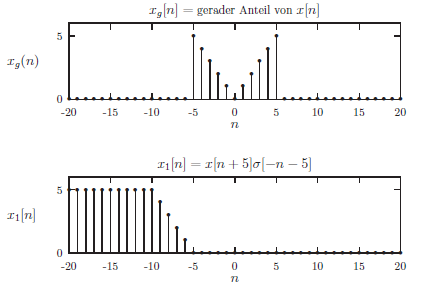
\includegraphics{1_2}
	\end{center}
\subsection*{Lösung}
	In diesem Beispiel wird der Einheitssprung $\sigma$ verwendet. Dieser ist definiert mit
	\[
		\sigma\leftn[n\right]=\left\{\begin{array}{cl} 0, & n<0\\1, & n\ge 0 \end{array} \right.
	\]
	Betrachten wir nun die Funktion $x_1\leftn[n+5\right]\sigma \leftn[-n-5\right]$, lässt sich leicht erkennen, dass der Einheitssprung $\sigma \leftn[-n-5\right]$ nur bei $n\le -5$ Werte zulässt. Wir können das Signal $x\leftn[n\right]$ vorerst nur bis zu dieser Stelle rekonstruieren.\\
	Der Ausdruck $x\leftn[n+5\right]$ verschiebt das Signal $x\leftn[n\right]$ nach links. Es lässt sich aus dem Plot herauslesen, dass $x\leftn[n\right]$ bis zu $n=-5$ den Wert $5$ erzeugt, und anschließend linear von -5 gegen 0 abfällt. Wir können definieren:
	\[
		x\leftn[n\right]=\left\{\begin{array}{cl} 5, & n < -5\\-n, & -5\le n<0\\?, & n\ge 0 \end{array} \right.
	\]
	Nun fehlt uns noch Definition für positive n-Werte. Dabei bedienen wir uns dem angegebenen $x_g\leftn[n\right]$ und der Umformung:
	\[
		x_g\leftn[n\right]=\frac{1}{2} \left(x\leftn[n\right]+x\leftn[-n\right]\right)\Leftrightarrow x\leftn[n\right]=2x_g\leftn[n\right]-x\leftn[-n\right]
	\]
	Das heißt, dass wir alle positiven Signalwerte von $x\leftn[n\right]$ berechnen können, indem wir die geraden Anteile $x_g\leftn[n\right]$ und die negativen Signalwerte $x\leftn[-n\right]$ kennen. Nun muss nur noch der Parameter $n$ für $n \ge 0$ variiert werden.
	\begin{center}
		\begin{tabular}{|c|c|c|c|c|c|c|c|c|c|c|c|}
		\hline n & 0 & 1 & 2 & 3 & 4 & 5 & 6 & 7 & 8 & 9 & 10 \\
		\hline $2x_g\leftn[n\right]$ & 0 & 2 & 4 & 6 & 8 & 10 & 0 & 0 & 0 & 0 & 0 \\
		\hline $x\leftn[-n\right]$ & 0 & 1 & 2 & 3 & 4 & 5 & 5 & 5 & 5 & 5 & 5 \\
		\hline $x\leftn[n\right]$ & 0 & 1 & 2 & 3 & 4 & 5 & -5 & -5 & -5 & -5 & -5 \\ 
		\hline 
		\end{tabular} 
	\end{center}
	Somit können wir $x\leftn[n\right]$ vollständig definieren:
	\[
		x\leftn[n\right]=\left\{\begin{array}{cl} 5, & n < -5\\|n|, & -5 \le n\le 5\\-5, & n>5 \end{array} \right.
	\]
	\begin{figure}[!h]	%1.2) x[n]
	\centering
		\begin{tikzpicture}[scale=0.5]
			\begin{axis}[
				xmin=-12, xmax=12,
				domain=-10:10,
				axis x line=middle,
				axis y line=middle,
				ylabel = {$x\leftn[n\right]$},
				y label style={at={(0.3,1)}},
				xlabel = $n$,
	       		xtick={-10,-5,...,10},
				]
				\addplot+[ycomb,blue,thick,domain=-10:-6,samples=5,mark=o] {5};
				\addplot+[ycomb,blue,thick,domain=-5:0,samples=6,mark=o] {-x};
				\addplot+[ycomb,blue,thick,domain=1:5,samples=5,mark=o] {x};
				\addplot+[ycomb,blue,thick,domain=6:10,samples=5,mark=o] {-5};
			\end{axis}
		\end{tikzpicture}
	\end{figure}
	Im letzten Schritt berechnen wir uns nun die ungeraden Teilsignale $x_u\leftn[n\right]$.
	\[
		x_u\leftn[n\right]=\frac{1}{2} \left(x\leftn[n\right]-x\leftn[-n\right]\right)
	\]
	Daraus erhalten wir:
	\[
		x_u\leftn[n\right]=\left\{\begin{array}{cl} 5, & -5 < n\\0, & -5\le n \le 5\\-5, & 5<n \end{array} \right.
	\]
	\begin{figure}[!h]	%1.2) x_u[n]
	\centering
		\begin{tikzpicture}[scale=1]
			\begin{axis}[
				xmin=-12, xmax=12,
				domain=-10:10,
				axis x line=middle,
				axis y line=middle,
				ylabel = {$x_u\leftn[n\right]$},
				y label style={at={(0.3,1)}},
				xlabel = $n$,
	       		xtick={-10,-5,...,10},
				]
				\addplot+[ycomb,blue,thick,domain=-10:-6,samples=5,mark=o] {5};
				\addplot+[ycomb,blue,thick,domain=-5:5,samples=11,mark=o] {0};
				\addplot+[ycomb,blue,thick,domain=6:10,samples=5,mark=o] {-5};
			\end{axis}
		\end{tikzpicture}
	\end{figure}
\section*{Aufgabe 1.3}
Jedes Signal $x\leftn[n\right]$ kann in ein gerades Signal $x_g\leftn[n\right]$ und in ein ungerades Signal $x_u\leftn[n\right]$ zerlegt werden. Zeigen Sie allgemein, dass
	\begin{enumerate}[a)]
		\item das Produkt $x_g\leftn[n\right]x_u\leftn[n\right]$ ein ungerades Signal ist
			\begin{align*}
				x_g\leftn[n\right] &=\frac{1}{2}\left(x\leftn[n\right]+x\leftn[-n\right]\right)\\
				x_u\leftn[n\right] &=\frac{1}{2}\left(x\leftn[n\right]-x\leftn[-n\right]\right)
			\end{align*} \begin{align*}
				x_g\leftn[n\right] x_u\leftn[n\right]&=\frac{1}{2}\left(x\leftn[n\right]-x\leftn[-n\right]\right)\cdot \frac{1}{2}\leftn(x\leftn[n\right]-x\leftn[-n\right]\right)\\
				&=\frac{1}{4}\left(x\leftn[n\right]+x\leftn[-n\right]\right)\cdot \left(x\leftn[n\right]-x\leftn[-n\right]\right)\\
				&=\frac{1}{4}\left(x\leftn[n\right]^2-x\leftn[-n\right]^2\right)
			\end{align*}
			Das ist dieselbe Form, wie ein ungerades Signal. Genauer gesagt, ist das das ungerade Teilsignal von $\frac{x\leftn[n\right]^2}{2}$.
		\item für das ungerade Signal gilt:
		\[
			\sum_{n=-\infty}^{\infty}x_u\leftn[n\right]=0
		\]
		Dafür spalte ich die Summe in drei Teile:
		\[
			\sum_{n=-\infty}^{-1}x_u\leftn[n\right]+x_u\leftn[0\right]+\sum_{n=1}^{\infty}x_u\leftn[n\right]
		\]
		Die erste Summe lässt sich mithilfe einer Indexverschiebung umschreiben:
		\[
			\sum_{n=-\infty}^{-1}x_u\leftn[n\right]=\sum_{n=1}^{\infty}x_u\leftn[-n\right]
		\]
		Eine Eigenschaft von ungeraden Signalen ist:
		\[
			x_u\leftn[-n\right]=-x_u\leftn[n\right]
		\]
		Das übernehmen wir nun für die Summe und erhalten:
		\[
			\sum_{n=-\infty}^{-1}x_u\leftn[n\right]+x_u\leftn[0\right]+\sum_{n=1}^{\infty}x_u\leftn[n\right]=x_u\leftn[0\right]+\sum_{n=1}^{\infty}x_u\leftn[n\right]-\sum_{n=1}^{\infty}x_u\leftn[n\right]
		\]\clearpage
		\item die Signalenergie gegeben ist durch
		\[
			\sum_{n=-\infty}^{\infty}x^2\leftn[n\right]=\sum_{n=-\infty}^{\infty}x_g^2\leftn[n\right]+\sum_{n=-\infty}^{\infty}x_u^2\leftn[n\right]
		\]
		Dafür setzen wir für $x\leftn[n\right]$ die Eigenschaft $x\leftn[n\right]=x_g\leftn[n\right]+x_u\leftn[n\right]$ ein:
		\[
			\sum_{n=-\infty}^{\infty}x^2\leftn[n\right]=\sum_{n=-\infty}^{\infty}\left(x_g\leftn[n\right]+x_u\leftn[n\right]\right)^2=\sum_{n=-\infty}^{\infty}\left(x_g^2\leftn[n\right]+2x_g\leftn[n\right]x_u\leftn[n\right]+x_u^2\leftn[n\right]\right)
		\]
		Nun müssen wir nur noch beweisen, dass $\sum_{n=-\infty}^{\infty}2x_g\leftn[n\right]x_u\leftn[n\right]=0$ gilt. Dafür ziehe ich die 2 aus der Summe und spalte sie auf:
		\[
			\sum_{n=-\infty}^{\infty}2x_g\leftn[n\right]x_u\leftn[n\right]=2\left(\sum_{n=-\infty}^{-1}x_g\leftn[n\right]x_u\leftn[n\right]+x_g\leftn[0\right]x_u\leftn[0\right]+\sum_{n=1}^{\infty}x_g\leftn[n\right]x_u\leftn[n\right]\right)
		\]
		Nun bedienen wir uns den Beweisen aus Aufgabe a und b. Durch a) wissen wir, dass die Multiplikation von einem geraden mit einem ungeraden Signal ein ungerades Signal ergibt. Im Punkt b) haben wir bewiesen, dass die unendliche Summe über ein ungerades Signal gleich 0 ist. Somit verschwinden diese drei Therme und es bleibt:
		\[
			\sum_{n=-\infty}^{\infty}x^2\leftn[n\right]=\sum_{n=-\infty}^{\infty}x_g^2\leftn[n\right]+\sum_{n=-\infty}^{\infty}x_u^2\leftn[n\right]
		\]
	\end{enumerate}
\section*{Aufgabe 1.4}

\subsection*{Angabe}
 
Welche Grundperiode hat das zeitdiskrete Signal
\[
	x\leftn[n\right]=e^{j\frac{2\pi}{N}nk}
\]
in Abhängigkeit von den ganzzahligen Größen $k$ und $N$?

\subsection*{Lösung}
Für ein periodisches Signal $x\leftn[n\right]$ mit der Periode $N$ gilt allgemein
\[
	x\leftn[n\right]=x\leftn[n+m\cdot N\right], \; m\in \mathbb{Z}
\]
Wenden wir nun diese Eigenschaft auf unser zeitdiskretes Signal an:
\begin{align*}
	x\leftn[n+N\right] &= e^{j\frac{2\pi}{N}(n+N)k}\\
	&= e^{j\frac{2\pi}{N}nk}e^{j\frac{2\pi}{N}Nk}\\
	&= e^{j\frac{2\pi}{N}nk}\underbrace{e^{j2\pi k}}_{=1}\\
	&= e^{j\frac{2\pi}{N}nk}
\end{align*}
In der Funktion bezeichnen wir $N$ als die \textbf{Periodendauer der Grundfrequenz}. Durch die Variation von $k=0,1,...,N-1$ erzeugen wir ganzzahlige Vielfache der Grundfrequenz, also harmonische Exponentialschwingungen bzw. Oberschwingungen.
\section*{Aufgabe 1.5}
\subsection*{Angabe}
Das Signal $x\leftn[n\right]$ sei periodisch mit der Periode $N$. Prüfen Sie, ob das Signal $y\leftn[n\right]=x\leftn[Mn\right]$ ($M$ ganzzahlig) ebenfalls periodisch ist. Bestimmen Sie gegebenenfalls die Periode von $y\leftn[n\right]$.
\subsection*{Lösung}
Das Signal $y\leftn[n\right]$ ist auf jeden Fall periodisch. Für die Ermittlung der neuen Periode betrachten wir folgendes Beispielsignal:
	\begin{figure}[!h]	%1.2) x_u[n]
	\centering
		\begin{tikzpicture}[scale=0.6]
			\begin{axis}[
				xmin=0, xmax=30,
				domain=0:30,
				axis x line=middle,
				axis y line=left,
				ylabel = {$x\leftn[n\right]$},
				y label style={at={(0.05,0.9)}},
				xlabel = $n$,
	       		xtick={0,5,...,30},
				]
				\addplot+[ycomb,blue,thick,domain=0:1,samples=31,mark=o] table {1_5_csv.csv};
			\end{axis}
		\end{tikzpicture}
	\end{figure}\\
Das Signal besitzt offensichtlich die Periode $N=10$. Nun wählen wir $M=2$ und erhalten:
	\begin{figure}[!h]	%1.2) x_u[n]
	\centering
		\begin{tikzpicture}[scale=0.6]
			\begin{axis}[
				xmin=0, xmax=30,
				domain=0:30,
				axis x line=middle,
				axis y line=left,
				ylabel = {$y\leftn[n\right]=x\leftn[2n\right]$},
				y label style={at={(0.03,0.7)}},
				xlabel = $n$,
	       		xtick={0,5,...,30},
				]
				\addplot+[ycomb,blue,thick,domain=0:1,samples=31,mark=o] table {1_5_csv2.csv};
			\end{axis}
		\end{tikzpicture}
	\end{figure}\\
Wir wählen nur jeden zweiten Wert, unsere Periode verkürzt sich auf $N=5$. Dasselbe führen wir mit $M=3$ durch:
	\begin{figure}[!h]	%1.2) x_u[n]
	\centering
		\begin{tikzpicture}[scale=0.6]
			\begin{axis}[
				xmin=0, xmax=30,
				domain=0:30,
				axis x line=middle,
				axis y line=left,
				ylabel = {$y\leftn[n\right]=x\leftn[3n\right]$},
				y label style={at={(0.03,0.7)}},
				xlabel = $n$,
	       		xtick={0,5,...,30},
				]
				\addplot+[ycomb,blue,thick,domain=0:1,samples=31,mark=o] table {1_5_csv3.csv};
			\end{axis}
		\end{tikzpicture}
	\end{figure}\\
Hier wird nur jeder dritte Wert verwendet. Die Periode ist diesesmal $N=10$. Die Formel lautet
\begin{center}
	$N_x=\frac{N}{ggT(N,k)}$
\end{center}
\section*{Aufgabe 1.6}
\subsection*{Angabe}
Die Fourierreihendarstellungen der periodischen Signale $x\leftn[n\right]$ und $y\leftn[n\right]$ sind gegeben durch
\[
	x\leftn[n\right]=\sum_{k=0}^{N-1}c_ke^{j\frac{2\pi}{N}nk}\Leftrightarrow c_k=\frac{1}{N}\sum_{n=0}^{N-1}x\leftn[n\right]e^{-j\frac{2\pi}{N}nk}
\]
und
\[
	y\leftn[n\right]=\sum_{k=0}^{N-1}d_ke^{j\frac{2\pi}{N}nk}\Leftrightarrow d_k=\frac{1}{N}\sum_{n=0}^{N-1}y\leftn[n\right]e^{-j\frac{2\pi}{N}nk}
\]
Berechnen Sie den Zusammenhang zwischen den Fourierreihenkoeffizienten $d_k$ und $c_k$ für die folgenden Signalbeziehungen:
\begin{enumerate}[a)]
	\item $y\leftn[n\right]=x\leftn[n-\frac{N}{2}\right]$,	$N$ gerade
	\item $y\leftn[n\right]=x\leftn[N-n\right]$
	\item $y\leftn[n\right]=\frac{1}{2}\left(x\leftn[n\right]+x^*\leftn[N-n\right]\right)$
	\item $y\leftn[n\right]=x\leftn[2n\right]$
	\item $y\leftn[n\right]=x\leftn[n\right]cos \frac{2\pi L}{M}n$,	$L$ und $M$ ganzzahlig
	\item $y\leftn[n\right]=x^2\leftn[n\right]$
\end{enumerate}
\subsection*{Lösung}
\section*{Aufgabe 1.7}
\subsection*{Angabe}
Für die gegebenen periodischen Signale bestimme man die Fourierreihenkoeffizienten $c_k$:
\begin{enumerate}[a)]
	\item $x\leftn[n\right]=1-cos\frac{\pi}{4}n$
	\item $x\leftn[n\right]=\left(\frac{1}{2}\right)^n, -2\le n\le 3$, und $x\leftn[n+6\right]=x\leftn[n\right]$
	\item $x\leftn[n\right]=\sum\limits_{k=-\infty}^{\infty}\delta \leftn[n-3k\right]$
\end{enumerate}
\subsection*{Lösung}
Für die Fourierreihenkoeffizienten $c_k$ gilt:
\[
	c_k=\frac{1}{N}\sum_{n=0}^{N-1}x\leftn[n\right]e^{-j\frac{2\pi}{N}kn}, \; k=0,1,...,N-1
\]
Außerdem hilft uns die Summenformel der endlichen geometrischen Reihe weiter:
\[
	\sum_{k=0}^{N-1}x^k=\frac{1-x^N}{1-x}
\]
\begin{enumerate}[a)]
	\item $x\leftn[n\right]=1-cos\frac{\pi}{4}n$\\
	\begin{align*}
		c_k &= \frac{1}{N}\sum_{n=0}^{N-1}x\leftn[n\right]e^{-j\frac{2\pi}{N}kn}\\
		&= \frac{1}{N}\sum_{n=0}^{N-1}\left(1-cos\left(\frac{\pi}{4}n\right)\right)e^{-j\frac{2\pi}{N}kn}\\
		&= \frac{1}{N}\sum_{n=0}^{N-1}e^{-j\frac{2\pi}{N}kn}-\frac{1}{N}\sum_{n=0}^{N-1}cos\left(\frac{\pi}{4}n\right)e^{-j\frac{2\pi}{N}kn}
	\end{align*}
	Nun benutzen wir die Umformung
	\[
		cos(x)=\frac{1}{2}\left(e^{jx}+e^{-jx}\right)
	\]
	und erhalten:
	\begin{align*}
		c_k &= \frac{1}{N}\sum_{n=0}^{N-1}e^{-j\frac{2\pi}{N}kn}-\frac{1}{2N}\sum_{n=0}^{N-1}e^{j\frac{\pi}{4}n}e^{-j\frac{2\pi}{N}kn}-\frac{1}{2N}\sum_{n=0}^{N-1}e^{-j\frac{\pi}{4}n}e^{-j\frac{2\pi}{N}kn}\\
		&= \frac{1}{N}\sum_{n=0}^{N-1}e^{-j\frac{2\pi}{N}kn}-
		\frac{1}{2N}\sum_{n=0}^{N-1}e^{j\frac{2\pi}{N}n(\frac{N}{8}-k)}-
		\frac{1}{2N}\sum_{n=0}^{N-1}e^{j\frac{2\pi}{N}n(-\frac{N}{8}-k)}
	\end{align*}
	Nun wenden wir die Summenformel an und erhalten:
	\begin{align*}
		c_k &=
			\frac{1}{N} \frac{1-e^{-j2\pi k}}{1-e^{-j\frac{2\pi}{N}k}} -
			\frac{1}{2N} \frac{1-e^{j2\pi \left(N-k\right)}}{1-e^{j\frac{2\pi}{N} \left(N-k\right)}} -
			\frac{1}{2N} \frac{1-e^{j2\pi \left(-N-k\right)}}{1-e^{j\frac{2\pi}{N} \left(-N-k\right)}}
	\end{align*}
	Ich darf den Exponenten beliebig mit N erweitern (siehe Folie 26 - Handout 1):
	\begin{align*}
		c_k &=
			\frac{1}{N} \frac{1-e^{-j2\pi k}}{1-e^{-j\frac{2\pi}{N}k}} -
			\frac{1}{2N} \frac{1-e^{j2\pi \left(N-k\right)}}{1-e^{j\frac{2\pi}{N} \left(N-k\right)}} -
			\frac{1}{2N} \frac{1-e^{j2\pi \left(N-k\right)}}{1-e^{j\frac{2\pi}{N} \left(N-k\right)}}\\
			&=
			\frac{1}{N} \frac{1-e^{-j2\pi k}}{1-e^{-j\frac{2\pi}{N}k}} -
			\frac{1}{N} \frac{1-e^{j2\pi \left(N-k\right)}}{1-e^{j\frac{2\pi}{N} \left(N-k\right)}}
	\end{align*}
\end{enumerate}
\end{document}